\documentclass[german]{cgspaper} % change option to 'english' to include english logo in \copyrightspace

\usepackage[ngerman]{babel} % comment out to use english in auto-generated section titles
\usepackage[utf8]{inputenc}
\usepackage[ruled]{algorithm}
\usepackage{algpseudocode}
\usepackage{url}
\usepackage{color}
\usepackage{tabularx}

\definecolor{colorMartin}{RGB}{147,83,177}
\definecolor{colorPascal}{RGB}{255,127,0}
\definecolor{colorTobias}{RGB}{160,123,46}

\newcommand{\todo}[1]{\textit{#1}}
\newcommand{\Martin}[1]{\textcolor{colorMartin}{TODO Martin:} \todo{#1} }
\newcommand{\Pascal}[1]{\textcolor{colorPascal}{TODO Pascal:} \todo{#1} }
\newcommand{\Tobias}[1]{\textcolor{colorTobias}{TODO Tobias:} \todo{#1} }

\newcommand{\neuerBegriff}[1]{\textbf{\textit{#1}}}

\title{Selfaware Monopoly}
\author{Martin Fischer, Pascal Crenzin, Tobias Knöschke\\ Digital Engineering Fakultät, Hasso-Plattner-Institut \textbar{} Universität Potsdam}

% Konfiguration des Veranstaltungs-Feldes
\subject{%
    \textbf{Advanced Games of Life}\\
    Sommersemester 2018\\
    Themenstellung und Anleitung:
    Willy Scheibel, Stefan Buschmann und Prof.\ Dr.\ Jürgen Döllner}

\begin{document}

% Definition des Teasers
\teaser{
    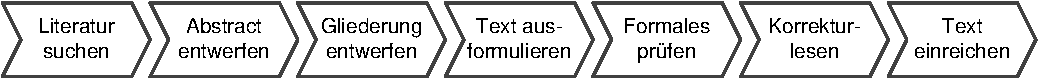
\includegraphics[width=0.9\textwidth]{graphics/prozess.pdf}
    \caption{Beispiel für einen Teaser: Schritte beim Erstellen eines fachwissenschaftlichen Beitrags. Ein Teaser dient als Blickfang schon auf der ersten Seite eines Artikels.}
    \label{fig:prozess}
}

\maketitle

%----------------------------------------------------------------
% Zusammenfassung
%----------------------------------------------------------------
\begin{abstract}
    \Martin{Zusammenfassung schreiben}
\end{abstract}

\copyrightspace % Erzeugt den Hinweis auf die Veranstaltung links unten


\section{Einleitung}

Informations Systeme ersetzen immer mehr elementare Bestandteile unserer Gesellschaft.
Soziale Netzwerke, das Finanz- und Bankwesen, Wahlsysteme um nur eine wenige Bereiche zu nennen.
Dabei Vertrauen alle Beteiligten darauf das diese Systeme sich an die Regeln halten und alle Beteiligeten gleichermaßen fair behandeln.

Was wäre wenn dies nicht der Fall ist? 
Was wäre wenn innerhalb des Systems Hintertüren existieren, welche es ermöglichen einzelne Regeln zu umgehen.
Was wäre wenn das System durch das benutzen dieser Hintertüren, die Grenzen seiner Spezifikation überschreitet und sich so Zugang zu Information und Ressourcen verschafft, welche es nicht besitzen dürfte.

Im Rahmen des Seminars Games of Life wollen wir ein solches System konzipieren und implementieren.

\section{Konzept}

Das Spiel Monopoly war urpsrünglich als Gesellschaftskritik am Kapitalismus gedacht. \Martin{Nachweis} 
Aufbauend auf dieser Grundidee wollen wir nun ein Spiel entwerfen, welches dem Spieler die Möglichkeit gibt die Spielregeln zu umgehen und sich im Gegenzug Information und Resourcen vom Spieler beschaft. 
Diese Komponente wird im folgenden \neuerBegriff{Watson} genannt.

\subsection{Watson}

Watson bietet den Spieler immer wieder die Möglichkeit, die Regel von Monopoly zu umgehen und dem Spieler so einen Vorteil zu verschaffen.
Im Gegenzug wird Watson versuchen unterschiedliche Ressourcen die nicht Inhalt des Spiels sind vom Spieler zu erhalten.
Ein solcher Handel wird im folgenden als \neuerBegriff{Deal} bezeichnet.
Die Spieler müssen aktiv die Entscheidung treffen, dass sie Watson nutzen.
Dadurch kann Watson nur so weit agieren, wie es die Spieler zulassen.
Sollte also alle Spieler eines Spiels zu keiner Zeit die Deals von Watson annehmen, entspricht das Spiel eine regelkonformen Monopolypartie.

\subsubsection{Was will Watson?}

Watson interessieren persöhnliche Information, Ressourcen und die Nutzung der Identität der Spieler um in ihrem Namen aufzutreten.

Persöhnlich Informationen die Watson bekommen möchte sind zum Beispiel die Identität des Spielers auf Facebook, Twitter oder anderen Sozialen Platformen und das Scannen von E-Mails.
\Pascal{Welche Plattformen und E-Mail accounts?}

Ressourcen die Watson bekommen möchte ist Rechnenleistung um Bitcoinmining zu betreiben.
Beim Bitcoinmining wird die Kryptowhärung Monero gemined.

Watson möchte die Identität der Spieler nutzen um auf Socialen Plattformen Likes oder Kommentare zu erstellen.
\Pascal{Welche möglichkeiten haben wir umgesetzt?}

\subsubsection{Wie sieht so ein Deal aus?}

Watson bietet dem Spieler unterscheidliche Deals an die Regeln zu umgehen.

\begin{table}[h]
\centering
\begin{tabular}{|c|c|c|}
\hline 
& \textbf{verdeckt} & \textbf{offen} \\
\hline
\textbf{direkt} & Würfel manipulieren & - \\
\hline
\textbf{indirekt} & Glück beeinflussen & Baupreis reduzieren \\
\hline
\end{tabular}
\caption{Die Tabelle kategorisiert die Effekte der Deals, die durch Watson angeboten werden, in zwei Dimensionen. In der horizontalen ob der Effekt eines Deals für die Spieler sichtbar ist und in der verticallen ob der Effekt direkt eintritt.}
\label{tab:effekte}
\end{table}

Tabelle \ref{tab:effekte} kategorisiert die Effekte eines Deals in zwei Dimensionen, direkt oder indirekt, das bedeutet ob der Spieler ein direkt Nutzen bekommt und in offensichtlich und nicht offensichtlich.
Daraus ergeben sich strukturell folgen Deals.

\neuerBegriff{Offensichtlich-direkt} wäre ein offensichtlicher Deal, wie der Spieler darf Geld aus der Bank nehmen und gibt dafür Informationen von sich preis. 
Da es in dem Scenario nicht darum geht, wer am skrupelosesten schummelt, wird diese Art von Deals nicht durch Watson angeboten.

\neuerBegriff{Offensichtlich-indirekt} sind alle Deals, bei denen andere Spieler den Effekte als Regelbruch ausmachen können aber die nicht direkt beim Preisgeben von Informationen oder Ressourcen einen Effekt haben.
Der Spieler weis zu den Zeitpunkt wenn ihm der Deal angeboten wird nicht nicht ob er, die Leistung durch Watson braucht oder nicht.
Dadurch soll der Spieler zum Hammstern angehalten werden und im Zweifel mehr von sich Preis zu geben als nötig wäre.

Watson bietet den Spieler zum Beispiel an, Bitcoin Mining zu betreiben und so für jede Spielrunde die da Bitcoin-Mining im Hintergrund läuft, einen so genannten \neuerBegriff{Watson-Coin} zu generieren.
Die Watson-Coins werden dann durch Watson für jeden Spieler ein Konto gespeichert.
Der konkrete Stand dieses Kontos ist für den Spieler aber nicht einsehbar.
Baut ein Spieler der Watson-Coins besitzt Häuser, so wird der Preis pro Watson-Coin um 50.
Das tatsächlich erwirschaftete Guthaben auf Monero geht an Watson, bzw an das System.
Für andere Spieler ist es nur beim Hausbau einsehbar ob der Spieler einen Deal von Watson angenommen hat oder nicht.
Die Zahlen werden innerhalb des Spiels aber nur durch genaues hinschauen und nachrechnen einsehbar sein, wodurch es erschwert ist dies von außen mitzubekommen. 

\neuerBegriff{verdeckt-direkt} sind alle Deals, bei denen der Spieler Information oder Ressourcen an Watson übergibt und einen direkten Nutzen davon hat. 
Durch den direkten Mehrwert den der Spieler gezeigt bekommt, soll der Spieler in Versuchung gebracht werden, selbst wenn er eigentlich keine Deals annehmen möchte, dies an dieser Stelle doch zu tun.
Zum Beispiel ist es gerade im frühen und im späten Spielverlauf von entscheidender Bedeutung, entweder unbedingt oder auf keinen Fall ein bestimmtes Würfelergebniss zu erzielen.

Watson bietet deshalb den Spieler an die Würfel zu manipulieren.
\Pascal{Sind das noch weitere Deals?}
Der Spieler muss dafür seine Identität auf Facebook an Watson übergeben und darf sich so sein nächstes Würfelergebniss wählen.
Für andere Spieler ist es in keiner Weise einsichtig ob der Spieler einen Deal von Watson angenommen hat oder nicht.

\neuerBegriff{verdeckt-indirekt} sind alle Deals, bei denen der Spieler Information oder Ressourcen an Watson übergibt aber keinen direkten Effekt hat.
Der Spieler weiß dabei nicht einmal ob es überhaupt einen Effekt hat.
Da der Effekt nicht einmal für den Spieler selbst auszumachen ist, haben andere Spieler keine Möglichkeit herrauszufinden ob der Spieler Deals von Watson annimmt oder nicht.

Watson bietet den Spielern zum Beispiel an bestimmte Webseiten zu besuchen oder Kommentare und Seiten auf Facebook zu liken.
Tut der Spieler dies, merkt sich Watson dies und beeinflusst die Ereignisskarten die ein Spieler bekommt wenn er auf eine Ereignissfeld läuft.
\Pascal{Welcher Auslöser ist das genau?}

\subsubsection{Wann bietet Watson Deals an?}

Es ist wichtig das Watson zum einen für andere Spieler nicht merklich in den Spielfluss eingreift.
Das heißt wenn ein Spieler mit Watson interagiert sollen es die anderen Spieler nicht mitbekommen.
Dafür sollte Watson möglichst dann die Deals anbieten wenn der Spieler gerade nichts zu tun hat.
Deshalb bietet Watson Deals eher Spieler an, die gerade nicht an der Reihe sind.

Zum anderen soll Watson eine hohe Erfolgsrate haben, das heißt, die Wahrscheinlichkeit das ein Spieler den Deal annimmt soll hoch sein.
Um dies zu erreichen muss auf unterschiedlichste Faktoren geachtet werden. 

Es wird bestimmt, ob der Spieler den Effekt des Deals gebrauchen kann oder nicht. 
Einem Spieler der sehr viele Straßen besitzt, anzubieten die Würfel zu manipulieren hat wahrscheinlich weniger Erfolgschancen, als einem Spieler der unbedingt diese eine Straße brauch.
Einem Spieler mit einem unbebauten Straßenzug den Baupreis zu reduzieren, hat wahrscheinlich eine höhere Chance als einem Spieler ohne Straßen.

Spieler die schon Deals angenommen haben sollen Verhältnissmäßig viele Deals angeboten werden.
Wohingegen Spieler die noch keine Deals angenommen haben weniger bis garkeine Angebote mehr bekommne.

Deals sollen sich durch nur temporäre Verfügbarkeit interessant machen.
Somit ist der Spieler angeregt selbst wenn er den Effekt erst später nutzen kann diesen auch anzunehmen.
Weil er im Zweifel nicht darauf verzichten will.

Außerdem sollen einige Deals zufällig angeboten werden.
Das heißt ein Spieler bekommt eigentlich einen Deal auf denen eine oder mehrere der definierten Kriterien nicht zustimmen.

\subsection{Wie bietet Watson die Deals an?}

Die Watson Komponente soll zwar Teil des Spiels sein aber für den Spieler soll Watson eine klar erkennbare Komponente innerhalb des Interfaces darstellen.
Dadurch soll klar werden, dass dies nicht mehr zu dem eigentlichen Monopolyspiel gehört und der Spieler an dieser Stelle eine Grenze überschreitet.
Der Spieler muss dadurch aktiv Entscheiden ob er diesen Teil des Spiels nutzt.

\section{Vorstellung Prototyp}

% Allgemein
Der Prototyp präsentiert sich dem Nutzer als Website, welche dieser in einem normales Webbrowser aufrufen kann.
Die Bereitstellung als Website bietet die Vorteile, dass einerseits jedweder Nutzer das Produkt nutzen kann, ohne dass spezielle Voraussetzungen, wie beispielsweise ein spezifisches Betriebssystem, gegeben sein müssen, während andererseits der Server als Anbieter unter bekannten und kontrollierbaren Bedingungen entwickelt werden kann.

Der Server selbst ist geteilt in einen HTML-Server, welcher die Websites bereitstellt, sowie einen Websocket-Server, welcher die Spiellogik, inklusive Manipulationen implementiert und Auskunft über Ereignisse in den laufenden Spielen gibt.
Diese beiden Komponenten sind zum großen Teil unabhängig. Die einzigen Verbindungen bestehen in der API, mit der über die Websockets kommuniziert wird, sowie dem Umstand, dass der Client die korrekte Adresse für die Verbindung zum Websocket kennen muss.
Entsprechend dieser klaren Aufteilung wurden die Implementierungen parallel von zwei getrennten Gruppen durchgeführt, aufbauend auf der gemeinsam genutzten Websocket API.

% Spielstatus
Da im finalen System mehrere Akteure zusammenwirken, kommt das Problem der Synchronisation auf. In diesem speziellen Fall müssen sich der Server und sämtliche an einem Spiel beteiligten Clients einig sein über den Zustand dieses Spiels.
Für jede Änderung einmal den vollständigen Zustand an sämtliche Clients zu senden wäre nicht nur eine zusätzliche Last für das Netzwerk, sondern auch ein erheblicher Mehraufwand für den Server, der zusätzlich dadurch erhöht wird, dass bedingt durch die Manipulationen von Watson manche Informationen nur bestimmten Spielern zugänglich sein dürfen.
Aus diesem Grund müssen sämtliche Teilnehmer eine eigene lokale Kopie des Zustandes vorhalten, welche sie bei Bedarf aktualisieren.
Der individuelle lokale Zustand wird ausgehend von einem Grundzustand iterativ durch Anwendung einzelner lokaler Aktionen erzeugt.
Während der Grundzustand einzig von der Anzahl der beteiligten Spieler, deren Namen und dem gewählten Spielbrett abhängt, behandeln die Aktionen sämtliche Änderungen, welche durch die Züge und Entscheidungen der Spieler entstehen.
Um inkrementellen Fehlern vorzubeugen, wird zum einen darauf geachtet, dass Aktionen in strikt der Reihenfolge angewendet werden, in der sie aufgetreten sind.
Zum anderen wird für jede Änderung eines Wertes nicht die relative Veränderung übermittelt, wie es vor allem für die Kontostände und die Positionen der Spielfiguren einleuchtend wäre, sondern das absolute Ergebnis der Aktion.

Die Abfolge der Aktionen wird für jedes Spiel in einer Datenbank hinterlegt, und ursprünglich erfolgte dies nur zur Dokumentation der mit dem Prototypen durchgeführten Nutzerstudien.
Später wurden diese Aufzeichnungen auch dafür verwendet, um es Spieler, die durch äußere Störungen die Verbindung zum Server verloren haben, zu ermöglichen, wieder in ihr Spiel einzusteigen und die ,,verpassten`` Aktionen nachzuholen.

% Server-Client-Kommunikation
Die Kommunikation über die Websockets erfolgt asynchron, da beide Kommunikationspartner Meldungen an den anderen machen können, welche meist keiner direkten Rückmeldung bedürfen.
Als Datenformat wurde JSON gewählt, da es einerseits von beiden Seiten einfach erzeugt und dekodiert werden kann, und andererseits selbst im ,,kodierten`` Zustand noch menschenlesbar und somit leichter nachvollziehbar ist.
Der Inhalt einer Nachricht besteht aus einem Feld für den Zweck sowie weiteren Informationen, sofern der diese für den Zweck relevant sind. Während beispielsweise die Meldung über das Ende des Spiels ohne weitere Parameter versendet werden kann, wäre eine Nachricht über die Bewegung eines Spielers ohne die Angabe des Ziels sinnlos.

Die Inhalte der Nachrichten reichen von organisatorischen Belangen, wie der Anmeldung eines Nutzers oder dem Beitritt zu einem Spiel, über spielinterne Geschehnisse, wie die Augenzahl der Würfel nach einem Wurf oder der Veränderung des Kontostands eines Spielers, bis hin zur Ausführung von Schummelaktionen, wie der Festlegung des nächsten Wurfergebnisses.
Während beide Kommunikationspartner spontan Nachrichten an den anderen schicken können, übernimmt der Client, also der Nutzer mit seinem Browser, eine aktivere Rolle als der Server.
Während der Server nur Statusmeldungen an die Clients schickt, wird ein Client bei bestimmten Anfragen auf spezifische Meldungen des Servers warten. Beispielsweise erwartet ein Client, der die Nachricht zum Kauf eines Grundstücks gesendet hat, dass einerseits der Besitzer dieses Grundstücks geändert wird, und sich andererseits der eigene Kontostand ändert.
Zu beachten ist, dass jede dieser Anfragen genauso gut mit einer Fehlermeldung beantwortet werden kann. Diese Fehlermeldungen handeln dabei von nicht durch Watson abgedeckten Regelverstößen, wie fehlende Besitzansprüche oder einen zu geringen Kontostand.

% Client-Architektur
Der HTML-Server stellt den Nutzer zwei verschiedene Webseiten bereit.
Die erste Seite, die ein Nutzer sieht, ist die Lobby, in der er sich erst einen Anzeigenamen aussuchen darf, und anschließend entweder einem bestehenden Spiel beitreten oder ein neues Spiel einleiten kann.
Die andere Seite behandelt eine konkrete Instanz des Spiels. Sie enthält Informationen über den Zustand des Spielbretts, die Besitztümer aller beteiligten Spieler, sowie eine Auflistung sämtlicher Aktionen, die der Nutzer ausführen kann.
Es liegt in der Natur dieser beiden Seiten, vor allem aber in der der zweiten Seite, dass sie dynamischen Inhalt zeigen müssen, der sich während der Betrachtung durch äußere Einflüsse ändern kann.
Diesen dynamischen Inhalt auf Serverseite einzusetzen und die fertige Seite an den Client zu senden, hätte nicht nur dazu geführt, dass sich die Seiten aufs Geratewohl erneut laden müssten, sondern auch den HTML-Server als Mittelsmann zwischen dem Client und dem für die Spiellogik verantwortlichen Server eingesetzt.
Stattdessen werden beide Seiten mit einem statischen Grundgerüst ausgeliefert, welches mittels Skripten zuerst eine direkte Verbindung zum Websocket-Server aufbaut, um dann mit den von dort empfangenen Daten die eigentliche Seite aufzubauen.
Die Verwendung von Skripten und Websockets erlaubt nicht nur, die Aktualisierung der angezeigten Inhalte zu verzögern, bis auf dem Websocket tatsächlich neue Informationen eintreffen, sondern zusätzlich punktuelle Änderungen der betroffenen Abschnitte, ohne die Seite vollständig neu laden zu müssen.

Für die dynamische Anpassung der Seiten kommt das Framework Vue\footnote{https://vuejs.org} zum Einsatz.
Es erlaubt, die Struktur des HTML-Dokuments und die Eigenschaften seiner Elemente an Skript-Variablen zu binden, sodass sich der Inhalt nach dem Wert der Variablen richtet.
Zusätzlich werden Callbacks eingerichtet, mit denen sämtliche von einer Variablen abhängigen Elemente automatisch aktualisiert werden, sobald sich der Wert der Variablen ändert.
Dies geschieht separat für alle gebundenen Variablen, sodass der Aufwand für die Aktualisierung gering gehalten wird.
Zusätzlich werden vielerorts die mit HTML 5 eingeführten Templates\footnote{https://www.w3.org/TR/html50/scripting-1.html\#the-template-element} verwendet.
HTML-Templates erlauben es, HTML-Strukturen zu definieren, welche kopiert und angepasst werden können, bevor sie in das sichtbare Dokument eingefügt werden.
Durch das Zusammenwirken von Templates und den Manipulationen durch Vue erhalten die Seiten einen ausgeprägten objektorientierten Charakter.

% Server-Architektur
Die Architektur des Websocket-Servers basiert auf Modell des erweiterten endlichen Automaten.
Jedes laufende Spiel wird dabei durch einen Automaten modelliert, welcher auf Basis der von den Clients empfangenen Eingaben Zustandsänderungen vollführt und Ausgaben erzeugt.
Während das Spielfeld und die Besitztümer der Spieler in jederzeit erreichbaren Variablen gehalten werden, werden die Zustände des Automaten überwiegend durch die verschiedenen Phasen während des Zuges eines Spielers bestimmt.
Diese Zustände bestimmen die Auswahl an Aktionen, die die Spieler zum entsprechenden Zeitpunkt ausführen können, und basieren dabei auf den Regeln des Spiels.
Beispielsweise darf ausschließlich der Spieler, der gerade am Zug ist, würfeln, und dies auch nur, wenn er seinen Zug gerade begonnen hat oder durch einen Pasch erneut würfeln darf.
Zustandsübergänge erfolgen abhängig von den Aktionen der Spieler und dem aktuellen Spielstand, und folgen ebenfalls den Spielregeln.
Die Modellierung mittels Zuständen erlaubt eine übersichtliche Implementierung einzelner Aktionen, und schützt gleichzeitig davor, ungültige Aktionen zu unternehmen.

Während die Spiellogik mit dem genannten Automatenmodell von Grund auf implementiert wurde, wurden für die Kommunikation mit den Clients entsprechende Bibliotheken benutzt.
Speziell finden einige Komponenten des Frameworks Qt\footnote{https://qt.io} Anwendung.
Qt bietet neben einer Implementierung von Websockets auch die Möglichkeit zur asynchronen Kommunikation mittels Signalen und einer Event Queue, wovon in Bezug auf das Versenden der Rückmeldungen an die Clients Gebrauch gemacht wurde.
Für die Datenbank, in der sowohl die Spieler als auch sämtliche Spiele inklusive ihrer Abläufe hinterlegt werden, bietet Qt eine Auswahl von Komponenten, welche die Verwendung einer SQL-Datenbank erleichtern.

% Watson
Die Schummelkomponente ,,Watson`` findet sich hauptsächlich im Client.
Während die Effekte, die Watson herbeiführt, im Server umgesetzt werden müssen, werden die Entscheidungen, ob und welche Angebote Watson dem Nutzer macht lokal im Client getroffen.
Auf der anderen Seite der Angebote, speziell bei der Anmeldung bei Dritten, besteht das Problem, dass nutzerspezifische Daten vom Client zum Server übertragen werden müssen.
Die Idee, die Zugangsdaten an den Server zu senden und über die API des Drittanbieters an entsprechende Zugangstokens zu gelangen, wurde davon abgelöst, den Client die Tokens direkt anfragen zu lassen, um diese dann an den Server zu senden.
Der letzte Schritt, das Senden an den Server, wird aus Sicherheitsgründen unterlassen. Für die Untersuchung des Verhaltens der Nutzer reicht der Erhalt der Tokens vom Drittanbieter aus.

Die Häufigkeit, mit der Angebote gestellt werden, sowie deren Inhalt hängt vom Zustand des Spiels und des Spielers ab.
Beispielsweise wird einem Spieler, dem zwei Grundstücke einer Farbgruppe gehören, während das dritte Grundstück noch nicht verkauft wurde, und der zusätzlich kurz vor dieser Farbgruppe steht, das Angebot gemacht werden, das Ergebnis seines nächsten Wurfs zu bestimmen.
Diese Regeln wurden willkürlich festgelegt und können mit der Einführung zusätzlicher möglicher Schummelaktionen erweitert werden.

Der Prototyp in seinem gegenwärtigen Zustand bildet nicht das vollständige Regelwerk eines handelsüblichen Monopoly ab, da einige teils elementare Bestandteile, wie Auktionen oder der Handel zwischen Spielern, fehlen.
Trotzdem ist er lauffähig, und dazu in der Lage, vollständige Spiele von Beginn bis Ende durchzuführen.
Aufgrund unvorhergesehener Verzögerungen war es nicht möglich, Nutzerstudien mit dem Prototypen durchzuführen.

\Pascal{Apis beschreiben}

Eine der Gegenleistungen, die für Schummelaktionen verlangt werden, ist die Verwendung von Rechnerressourcen des Nutzers, speziell für das sogenannte ,,Mining`` von Kryptowährung.
Um das Mining durchzuführen, werden Skripte von Coinhive\footnote{https://coinhive.com} in Anspruch genommen, welche die Währung Monero (XMR)\footnote{https://getmonero.org/} erzeugen.
Monero ist dem weitaus bekannteren Bitcoin sehr ähnlich, und steht zum Zeitpunkt des Verfassens dieser Ausarbeitung mit einem Wechselkurs von rund 113 USD zu 1 XMR im Kurs.

Das Mining für Monero erfolgt mittels einer Blockchain. Transaktionen, also Übertragungen von Monero von einem Besitzer zu einem Anderen, werden von den Minern in Blöcken verifiziert, und diese Blöcke der Blockchain angehängt.
Um übermäßiger Inflation vorzubeugen, wird die Erstellung gezielt künstlich erschwert, auf dass durchschnittlich nur ein einziger Block alle 2 Minuten entstehen kann.
Die künstliche Hürde besteht darin, einen Block zu generieren, dessen Hashwert unterhalb eines gewissen Schwellwerts liegt.
Jedem erfolgreich angefügten Block liegt ein stetig schrumpfender Bonus bei, der dem Erzeuger des Blocks gutgeschrieben wird.

Aufgrund der Seltenheit der Blöcke und der damit verbundenen Boni, ist das Konzept der ,,Pools`` entstanden.
Pools sind Zusammenschlüsse mehrerer Interessenten, die ihre Ressourcen zum Mining benutzen.
Erhält einer der Beteiligten den Bonus, wird er unter den Teilnehmern des Pool aufgeteilt.

Coinhive bietet einen derartigen Pool an, und nutzt mittels der bereitgestellten Skripte die Rechner Dritter für das Mining.
Die Boni aus erfolgreichen Blöcken behält Coinhive ein, zahlt aber demjenigen, der die Skripte auf seiner Seite einsetzt, einen kleinen Betrag pro Hashwert, den die von ihm ausgelieferten Skripte ausprobieren.
Die Höhe dieses Betrags hängt ab von der Wahrscheinlichkeit, einen gültigen Block zu erzeugen, und von der Höhe des Bonus, den der Block einbringen würde.

Laut Angaben von Coinhive zum Zeitpunkt der Schriftsetzung betrugen die Erfolgswahrscheinlichkeit rund 1 zu $7,155 \cdot 10^{12}$ und der Bonus pro Block rund 3,8 XMR.
Zudem geben sie an, ihre Skripte ließen auf hochwertigen Prozessoren rund 90 Hashwerte pro Sekunde berechnen.
Nimmt man all diese Zahlen, inklusive des Wechselkurses, zusammen, erhält man, dass ein einzelner Nutzer innerhalb einer Stunde einen Gegenwert von rund 0,000013 USD erzeugt.

\section{Diskussion}\label{sec:discussion}

Durch den Prototypen wurde gezeigt, das es möglich ist Systeme zu bauen, die versuchen den Nutzer mit seiner Zustimmung dazu zu bringen Infromation und Ressourcen von sich herzugeben ohne einen Mehrwert außerhalb des bereitgestellten Spiels zu gewähren.

Wir haben für die Diskussion drei relevante Themen indentifiziert.

\subsection{Hinter den API's}
Die API's einiger großen sozialer Plattformen wurden genutzt, um auf diesen nach Informationen zu suchen oder den Nutzer dazu zu bringen auf diesen im Interesse das Systems zu interagieren.
Alle API's dieser Plattformen haben bestimmte Schutz Mechanismen um sich vor böswilligen Handlungen zu schützen.

\Pascal{Was könnten man aber als Insider hinter den API's tun?}

\Pascal{Was wäre möglich wenn man die API's umgehen kann?}

\subsection{Analogie zu unserer Gesellschaft}

Innerhalb des Prototypens werden durch Watson immer wieder Möglichkeiten angeboten die allgemein geltenden Regeln zu umgehen.
In unserer Gesellschaft gelten genauso wie in dem Monopoly Spiel Regeln die für alle gültig sind.

Die durch Watson angeboten Deals wurden in 4 Kategorien eingeteil, wobei für den Prototyp nur drei von relevanz sind.
Alle diese Kategorien von Deals lassen sich auch in der wirklichen Welt finden.

\subsubsection{Verdeckte-Direkte Deals in der Gesellschaft}

Verdeckte-Direkte Deals sind Deals, bei dennen der Nutzten zwar verdeckt bleibt und es nicht klar ist, ob wirklich geschummelt wurde.
Innerhalb des Prototypens ist dies das Manipulieren des Würfelergebnisse. 
Analog dazu findet man in unserer Gesellschaft Schmiergeld, Bestechungen und Korruption.
Dabei werden Personen, Firmen oder Instutionen, welche in der Position sind Entscheidungen im Interesse aller zu treffen durch Geld oder Gegenleistungen beeinflusst.
Dies kann der bei Bau- oder Eventvergaben, bei politischen Entscheidungen oder aber auch das wegschauen bei einer ilegalen Handlung sein.
Im nachhinein ist es dann nur möglich anhand der Gegenleistung festzustellen ob es wirklich Bestechung bzw. Korruption war oder nicht.

Bestechung und Korruption sind überall in unserer Gesellschaft zu finden.
Sei es im Entertainment Sektor wie bei der Vergabe der Austragungsorte für die WM Frankreich und Südafrika wo es zu Korrupierung gekommen ist. \cite{FAZWM2015}

Innerhalb der Politik und selbst im der Exekutive ist Korruption ein Thema.
Zum Beispiel wurde jüngst Interpol-Chef Meng-Hongwei vor Bestechungsgelder angenommen zu haben. \cite{NTVINTERPOL2018}

So gennante PayToWin-Games sind bekannte vertreter von Informationssystemen, in welchen verdeckten-direkte Deals genutzt werden.
Bekannte Beispiele dafür sind Tribal Wars 2 oder Grepolis.
Die Spiele bieten dem Spieler die Möglichkeit, erweiterte Funktionalität und Inhalte des Spiels gegen Echtgeld zu erhalten.
Dabei kann der Spieler zum Beispiel nur eine beschränke Anzahl an Gebäuden in Auftrag geben.
Durch bezahlung Echtgeld kann er diese Beschränkung aufgehoben.
Dadurch hat er den Vorteil mit weniger Aufwand zu bauen.
Für andere Spieler ist es nicht einsichtig ob er dieses Feature in Anspruch nimmt oder nicht.

\subsubsection{Offene-Indirekte Deals in der Gesellschaft}

Offene-Indirekte Deals sind Deals, bei welchen der Nutzen für den Spieler verzögert eintritt und für andere Spieler erkenntlich ist das die Regeln umgangen wurden.
Im entwickelten Prototypen bietet Watson den Spielern an durch Bitcoin-Mining den Preis beim bau von Häusern zu reduzieren.

\Martin{Mapping Gesellschaft}

\Martin{Beispiel Gesellschaft}

\Martin{Beispiel Politik}

\Martin{Beispiel Informationssystem}

\subsubsection{Verdeckte-Indirekte Deals in der Gesellschaft}

Verdeckte-Indirekte Deals sind Deals, bei denen der Nutzen verzögert eintritt und auch nicht erkenntlich ist ob die Regeln umgangen wurden oder nicht.
Im entwickelten Prototypen ist es möglich durch besuchen von Websites die Ereignisskarten zu beeinflussen.
Folgt ein Spieler den durch Watson links, sorgt Watson dafür, dass es für den Spieler wahrscheinlicher ist positive Effekte durch Gemeinschafts- und Ereignisskarten zu erhalten.

\Martin{Mapping Gesellschaft}

\Martin{Beispiel Gesellschaft}

\Martin{Beispiel Politik}

\Martin{Beispiel Informationssystem}

\subsection{Warum baut man solche Systeme}

Wie in vorangegangen Teil des Kapitels \ref{sec:discussion} gezeigt wurde lassen sich alle implementierten Methodiken sowohl in bestehenden Software Systemen als auch in der Gesellschaft wiederfinden.

Dabei implementieren dieses Systeme meist nicht alle der Methodiken die im dem hier vorgestellten Prototyp gezeigt wurden, sondern nutzen eine Teilmenge mit einer der folgenenden Motivationen.

\subsubsection{Kapitalerzeugung}

Viele Systeme sind konzipiert um direkt Kapital zu erzeugen.
Manche davon nutzen die hier vorgestellten Methodiken um dies zu erreichen. 
Innerhalb der Computerspiele Industrie lasseb sich so gennante pay-to-win Spiele finden.
Diese ermöglichen es dem Spieler mit Echtgeld die Regel zu umgehen oder einen direkte Vorteil innerhalb des Spiels zu erkaufen.
Andere Spiel wie \Martin{Abstraction} aber auch Anwendungen wie \Martin{Sweat-Coin} nutzen Bitcoin-Mining um mit der Rechenleistung des Spielers Kapital zu generieren.

\subsubsection{Informationsbeschaffung}

Systeme welche das Ziel haben, Informationen über mögliche Kunden oder das Nutzungsverhalten von bestimmten Zielgruppen offen zu legen finden sich überall.
Die Teilmenge der Systeme, welche dafür einen Bonus oder Vorteil dem Nutzer geben, welche sonst nicht oder nur gegen Echtgeld erhältlich wären entsprechen der Methodik des Prototypen.
Beispiele dafür sind endlos, angefangen bei Gratiszeitungen gegen die eigene Anschrift bis hin zum verlinken des Facebook Accounts um einen Startbonus beim Anmelden auf einer Plattform zu bekommen.

\subsubsection{Meinungsverzehrung}

Beim Einkauf im Internet ist die Bewertung eines Produkts oft das wichtigste Kriterium ob man etwas kauft oder nicht.
Umso breiter das Spektrum der Bewerter desto eher vertraut man der Bewertung.
Änlich verhält es sich auch mit Bewertungen für Veranstaltung, Filme oder Restaurants.
Angenommen eine Firma will mehr oder bessere Berwertung machen ohne dies zu forcieren, kann das ein endlosses Unterfangen werden.
Deshalb wird versucht Nutzer zu einer Bewertung zu bewegen.
Ab dem Zeitpunkt wo der Nutzer für eine positive Bewertung eine Gegenleistung bekommt oder eine Berwertung vorgegeben wird verlässt man den legalen Bereich.

Wird die Identität einer anderen Person genutzt um einen Like oder eine Bewertung zu hinterlassen, ist dies gänzlich ilegal.
Facebook geht gegen so gennante FakeLikes aggressive vor.
Durch Facebook wird die im Prototyp umgesetzte Methode als Klickfarm bezeichnet. \cite{FakeLikes2018}

\section{Future Work}

Inhalt dieser Arbeit war es ein System zu erschaffen welches mit der aktiven Beteiligung der Nutzer bestimmte Regeln bricht und das System im Gegenzug versucht so viele Information und Ressourcen des Nutzers zu erhalten.

\subsection{Inteligente Watson Komponente}

Die Entscheidung wann welche Deals durch die Watson Komponente angeboten werden erfolgt momentan noch regelbasiert.
Watson könnte aber auch auf Grundlage von Metriken oder schon gewonnen Informationen agieren.
Dadurch könnte Watson versuchen mehr oder prisantere Informationen zu erhalten.
Außerdem könnte Watson auch Spiel übergreifend Interagieren.
Dadurch wäre auch das ableiten von Informationen möglich, wie zum Beispiel, wer spielt mit wem.
Ist es wahrscheinlich das sich diese Spieler auch außerhalb des Spiels kennen.
Wenn ja, könnte Watson einem der beiden Deals anbieten der beiden Spieler Hilft oder mit absicht dem anderem Spieler schadet.

\subsection{Persistenz}

Um den Prototypen sinnvoll für weitere wissenschaftliche Zwecke nutzten zu können, müssten die Spielverläufe persistiert werden.
Der Prototyp hält momentan alle Spielverläufe im Arbeitsspeicher.
Dies müsste um eine Persistierung auf eine Datenbank oder etwas vergleichbares erweitert werden.
Die Persistierung auf eine Datenbank würde den Vorteil bieten die Daten auch außerhalb des Prototyps zugänglich zu machen.

\subsection{Auswertung}

Nun stellen sich unterschiedlichste Fragen die mit Hilfe dieses Systems betrachtet werden können und sich dann auf unsere Gesellschafft übertragen lassen.
Solche Fragestellung könnten wie folgt aussehen?

\begin{itemize}
\item Ab wann empfindet der Spieler ein 'Schummeln' als legal/plausibel oder unrechtmäßig?
\item Wie regieren Gewinner des Spiels auf Belobung/Tadel?
\item Ändert sich die Einstellung der Spieler gegenüber dem Spiel abhängig vom Spielerfolg?
\item Inwiefern verändert sich die Bereitschaft zur Informationspreisgabe über den Verlauf des Spieles?
\item Bis zu welchem Grad ist ein Spieler bereit, bewusst zum Nachteil anderen Spieler zu agieren?
\end{itemize}

Um diese Fragen besser beantworten zu können, müssten die Aufgezeichneten Spieldaten analysiert und aufbereitet werden.
Zusätzlich müsste das Spiel um einen Feedback bzw. Fragemechanismus erweitert werden, der dem Spieler direkt nach dem Spiel Fragen über das Spielerlebniss stellt und diese mit den Daten über den Spielverlauf in Verbindung bringt.

\bibliographystyle{acmsiggraph}
\bibliography{gol-selfaware-monopoly}

\end{document}
